\documentclass{sig-alternate}

% UTF8 support
\usepackage[utf8x]{inputenc}


\usepackage{hyperref}
\usepackage{epsf,graphicx}
\graphicspath{{figures/}}
\usepackage{subfigure}
\usepackage[colorinlistoftodos]{todonotes}

\newcommand{\eg}{{\textit{e.g.~}}}
\newcommand{\etal}{{\textit{et al.~}}}
\newcommand{\ie}{{\textit{i.e.~}}}

%
% --- Author Metadata here ---
\conferenceinfo{10th ACM/IEEE International Conference on Human-Robot Interaction}{2015 Portland, USA}
%\CopyrightYear{2007} % Allows default copyright year (20XX) to be over-ridden - IF NEED BE.
%\crdata{0-12345-67-8/90/01}  % Allows default copyright data (0-89791-88-6/97/05) to be over-ridden - IF NEED BE.
% --- End of Author Metadata ---


\title{\LARGE \bf
``Those who can't do teach'': Learning Handwriting by Teaching a Robot
}


%%% HRI 2015 -> double-blind review process

%\numberofauthors{3} 
%\author{
%\alignauthor
%Deanna Hood\\
%Séverin Lemaignan\\
%Pierre Dillenbourg\\
%    \affaddr{Computer-Human Interaction in\\ Learning and Instruction (CHILI)}\\
%    \affaddr{Ecole Polytechnique Fédérale\\ de Lausanne (EPFL)}\\
%    \affaddr{CH-1015 Lausanne, Switzerland}\\
%    \email{firstname.lastname@epfl.ch}
%\alignauthor
%Rafael Garcia\\
%    \affaddr{Computer Vision and Robotics}\\
%    \affaddr{University of Girona}\\
%    \affaddr{Girona, Spain}
%}
%


\begin{document}



\maketitle

%%%%%%%%%%%%%%%%%%%%%%%%%%%%%%%%%%%%%%%%%%%%%%%%%%%%%%%%%%%%%%%%%%%%%%%%%%%%%%%%
\begin{abstract}

Despite the social motivation for the use of a teachable agent for the
engagement and support of children with handwriting difficulties, to date no
such technology is known to have been developed. Presented is a teachable
robotic agent in this context of handwriting skills acquisition. It is
hypothesised that such a system could not just engage an unmotivated student,
but could also present the opportunity for children to experience motor mimicry
during handwriting intervention. It also allows for exploring the potential for
the \emph{learning by teaching} paradigm to be employed in the interaction so as
to stimulate meta-cognition, empathy and increased self-esteem in the child
user. 

By leveraging simulated handwriting on a synchronised tablet display, a Nao
humanoid robot with limited fine motor capabilities has been configured as a
suitably embodied handwriting partner. Shape models derived from principal
component analysis of a dataset of letter trajectories are generated and allow
the robot to draw purposefully deformed letters. As a result, the objective of
developing an algorithm learning how to write characters well may be satisfied
by learning the optimal parameters for the model of said characters. Such a
learning algorithm has been developed, capable of incorporating feedback from
users both in terms of which generated letters are the best and from user
demonstrations. 

A pilot study, conducted to obtain insight into children's use of the system, is
presented, which has validated the interaction for an in situ experiment
scheduled with a primary school class to evaluate the human-robot interaction
outcomes of the system, the first of its kind. 

\end{abstract}


%%%%%%%%%%%%%%%%%%%%%%%%%%%%%%%%%%%%%%%%%%%%%%%%%%%%%%%%%%%%%%%%%%%%%%%%%%%%%%%%
\section{INTRODUCTION}

Handwriting difficulties in children at an early age often negatively affects
the academic performance of the students \cite{Christensen2005} in addition to
their self-esteem being adversely affected \cite{Malloy1995}, causing them to
shy away from expressing what they know \cite{Medwell2008}.
%A conclusion drawn
%in \cite{Hoy2011} is that any handwriting intervention studies considered in the
%systematic review which involved fewer than two practice sessions per week and
%fewer than a total of 20 practice sessions, including homework, were found to
%demonstrate ineffective results. This highlights the necessity to engage
%students in an interaction that will be sustainable over the long-term. 

Successful interventions for children with handwriting difficulties involve the
student in many sessions where they are engaged in physically practising the
skill \cite{Hoy2011}. However, the link between handwriting difficulties and low
self-efficacy \cite{Engel-Yeger2009} results in children who are unmotivated to
participate in such sessions, potentially leading to a developmental arrest in
the acquisition of the skill. 

%Engel-Yeger, Nagauker-Yanuv and Rosenblum \cite{Engel-Yeger2009} have shown the
%link between handwriting difficulties and low self-efficacy, the belief in
%one's capabilities to complete a task. Bandura \cite{Bandura1990} maintains
%that self-efficacy constitutes the basis for the choice of whether or not to
%attempt a task. Indeed, third graders receiving intervention for their
%handwriting skills in \cite{Berninger1997} spoke of how they avoid writing
%because of how it is illegible to others. This mindset of believing that one is
%unable to write may lead to a developmental arrest in the acquisition of this
%skill, which may make intervention more difficult in the future. Consequently,
%it is of importance to engage students in activities in which their
%self-efficacy and self-motivation is restored.

The learning by teaching paradigm, which engages the target student in the act
of teaching another, has been shown to produce motivational, meta-cognition, and
educational benefits in a range of disciplines \cite{Rohrbeck2003}. An
application which is yet to be explored, however, is the use of learning by
teaching in handwriting intervention. One reason why this may be the case is
that in order to engage a child in the learning by teaching paradigm, there must
be an appropriately unskilled peer for them to tutor. While in some cases it may
be appropriate for a peer or teacher to simulate a na\"ive learner, however this
acting is likely to be eventually detected if for an activity where one's skill
level is visually evident - as is the case in handwriting.

Presented is the development of the first known learning agent which is capable
of artificially making mistakes typical of children learning handwriting and
correcting them with external feedback, and therefore exhibiting the potential
to engage children in the learning by teaching paradigm in the context of
handwriting. Furthermore, the learning agent has been embodied in a commercially
affordable humanoid robot by leveraging synchronisation with a tablet display to
simulate fine motor skills otherwise infeasible for the robot. 

The significance in the learning by teaching paradigm of observing a teachable
agent respond to what has been taught \cite{Okita2006} is reasoning for using an
embodied agent which is capable of responding to handwriting feedback with a
process rather than simply a product. Therefore investigating the use of a
humanoid capable of executing handwriting trajectories is supported. The
potential for motor mimicry to yield significant improvements in handwriting
interventions \cite{Berninger1997} further supports the case for investigating
the use of a humanoid robot capable of physically demonstrating handwriting
trajectories to its child learning partner.

Section \ref{sec:learningAlgorithm} presents the learning algorithm employed for
developing a learning agent in the context of handwriting, Section
\ref{sec:robotWriting} details the extension of this algorithm to an embodied
robotic learning agent, and Section \ref{sec:experiment} explains the potential
use of such a system in addressing pedagogical research questions, as inferred
from experiments conducted with primary school children. 



%%%%%%%%%%%%%%%%%%%%%%%%%%%%%%%%%%%%%%%%%%%%%%%%%%%%%%%%%%%%%%%%%%%%%%%%%%%%%%%%
\section{A Learning Agent in the Context of Handwriting} \label{sec:learningAlgorithm}

Because of the objective to use an artificial intelligence algorithm in a
reinforcement learning framework, a parameterisation of letters and their
deformities has been sought such that, depending on the parameters input to the
letter models, different quality shapes can be generated: from bad, to good,
with the help of feedback from the reinforcement learning partner. To this end,
a method which can generate a model from real-world data has been employed in
order to capture said realistic variations. 

\subsection{Shape Modelling of Letters} \label{sec:writingGeneration}

One approach for a shape model which can appropriately represent realistic
variations in shapes with its parameters is statistical shape modelling, an
application of principle component analysis (PCA), where a linear transform that
de-correlates data vectors is found \cite{Stegmann2002}. 

PCA on a set of letter paths captured from a digital pen has been performed,
using the UJI Pen Characters 2 dataset \cite{Llorens2008} with 120 instances of
each letter (2 repetitions from 60 users). While it may be appropriate to
identify the location of the most salient features of the shapes in future work,
the features are currently taken as $n$ uniformly spaced points along the shape
path and arranged into an observation vector presented in (\ref{eq:obsVec}),
where $x_i$ and $y_i$ represent the coordinates of each of the points along the
path.

\begin{equation}\label{eq:obsVec}
{\bf x} = [x_1, x_2, \ldots, x_n, y_1, y_2, \ldots, y_n]^T
\end{equation}

In this work, the observation shapes are normalized such that they have a shape
centre of ${\bf 0}$ and a unit maximum dimension. 

The projection from the original $2n$ dimensional feature space to the $N$
dimensional feature space is then found as in (\ref{eq:projection}), where ${\bf
p}$ contains the coordinates in the $N$ dimensional space with ${\bf 0}$-origin,
calculated as in (\ref{eq:paramCalc}). The $2n\times N$ matrix ${\bf \Phi }$ is
an orthogonal matrix composed of the eigenvectors ${\bf v}_i$ of the covariance
matrix of the observations which correspond to the largest $N$ eigenvalues
($\lambda_i$), as shown in (\ref{eq:transformCalc}) \cite{Stegmann2002}. 

\begin{equation}\label{eq:projection}
{\bf \tilde{x}=\bar{x}+\Phi p}
\end{equation}
\begin{equation}\label{eq:paramCalc}
{\bf p} ={\bf \Phi}^T ({\bf {x}-\bar{x}})
\end{equation}
\begin{equation}\label{eq:transformCalc}
{\bf \Phi} = [{\bf v}_1, {\bf v}_2, \ldots, {\bf v}_N]^T
\end{equation}

If $N = 2n$, the projection will be nothing more than a change of basis, however
if there is correlation between the points in the observations, there will be
eigenvalues of the covariance matrix which are close to zero, and so removing
the associated eigenvectors from ${\bf \Phi}$ allows for dimensionality
reduction with minimal impact. Indeed, the amount of variance in the dataset
that is explained by each eigenvector ${\bf v}_i$ is $\sqrt{\lambda_i}$, and
therefore the proportion of the variance explained by each dimension/eigenvector
is as shown in (\ref{eq:proportionVar}).

\begin{equation}\label{eq:proportionVar}
\%var_i = \frac{\sqrt{\lambda_i}}{\sum_{i=1}^{N}\sqrt{\lambda_i}}\times 100\%
\end{equation}

Paths of a particular letter have been clustered using K-means clustering to
group different styles of writing the letter (\emph{allographs}), such that the
parameters in the resulting model are only representative of the specific
allograph of the letter in the dataset. PCA has been performed on all of the
paths of a particular allograph in the dataset at a time, to reduce the $2n$
dimensional space to one of a desired number of dimensions. This process may be
considered to generate a shape model in that (\ref{eq:projection}) may be used
to generate new shapes based on the parameters ${\bf p}$ which are used: ${\bf
p}={\bf 0}$ will yield the mean shape, and variations to each of the $N$ values
in ${\bf p}$ will cause a change in the shape represented by the corresponding
eigenvector (Figure \ref{fig:deviations_sPrint}). 

\begin{figure}[thpb]
\centering
\subfigure{
\raisebox{-0.5\height}{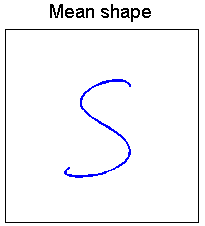
\includegraphics[width=0.07\textwidth]{figures/sPrint_mean.png}
}}
\subfigure{
\raisebox{-0.5\height}{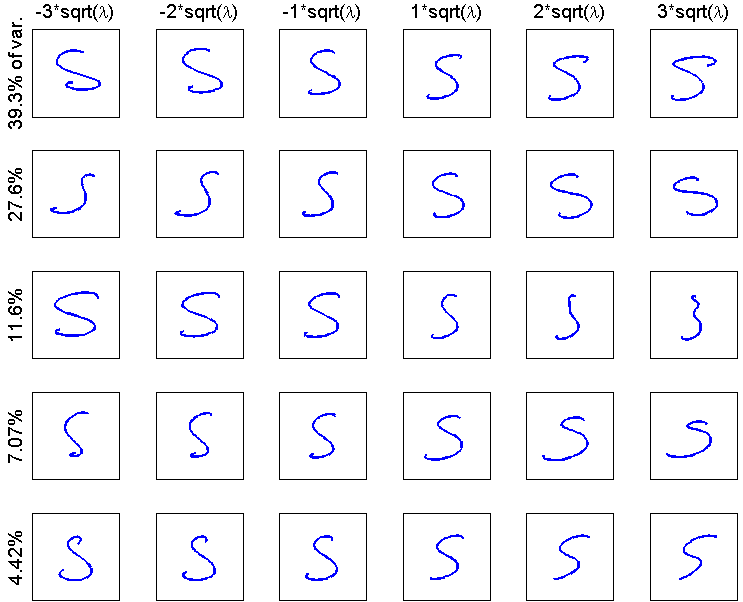
\includegraphics[width=0.38\textwidth]{figures/sPrint.png}
}}
\caption[The mean shape and the effect of varying the first five parameters of
the shape model derived from PCA from the dataset of print `s'
shapes.]{\label{fig:deviations_sPrint}The mean shape (left) and the effect
(right) of varying the first five parameters (each row) of the shape model
derived from PCA from the first cluster of `s' shapes, interpreted as the print
allograph. The percentage of the total variance in the dataset explained by each
parameter is shown on the appropriate row. }

\end{figure}

Interestingly, the parameters which result from the unsupervised statistical
shape analysis, to some extent, represent variations which could intuitively be
identified by a manual parameterisation: the gap in the top half of the letter
compared to the bottom half, the width of the top half of the letter compared to
the bottom half, the width of the overall shape, etc., and as a result the shape
modelling has produced the desired outcomes in terms of parameterising the
shapes in ways which are able to be used to deform them meaningfully.


\subsection{Generating Poor Letters}

After determining the appropriate number of dimensions (N) of the data
representing the majority of the variance observed within different samples of a
letter in the dataset, new letters can be generated by varying the parameter
values in this N dimensional space in accordance with (\ref{eq:projection}). By
choosing parameter values which lie within the observed range in the dataset, it
is possible to produce letters which are more likely to be reasonable looking.
When the parameter values are outside of the range observed in the dataset, they
are less likely to represent shapes from the dataset of reasonable,
adult-written letters, and as a result are more likely to represent poor shapes.
Figure \ref{fig:sampleLetters} illustrates sample letters generated from the
models of `e' and `g' - made from 120 observations with 70 points - by selecting
random values for the first 5 parameters from a distribution with standard
deviation of $3\sqrt\lambda_i$ rather than the $\sqrt\lambda_i$ standard
deviation observed in the dataset.

\begin{figure}[thpb]
\centering
\subfigure{\raisebox{-0.5\height}{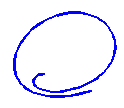
\includegraphics[height=0.08\textwidth]{figures/e1.png}}}
\subfigure{\raisebox{-0.5\height}{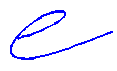
\includegraphics[height=0.05\textwidth]{figures/e4.png}}}
\subfigure{\raisebox{-0.5\height}{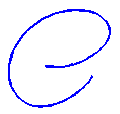
\includegraphics[height=0.08\textwidth]{figures/e3.png}}}
\subfigure{\raisebox{-0.5\height}{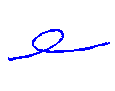
\includegraphics[height=0.08\textwidth]{figures/e5.png}}}\\
\subfigure{\raisebox{-0.5\height}{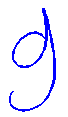
\includegraphics[height=0.12\textwidth]{figures/g1.png}}}
\subfigure{\raisebox{-0.5\height}{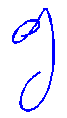
\includegraphics[height=0.12\textwidth]{figures/g3.png}}}
\subfigure{\raisebox{-0.5\height}{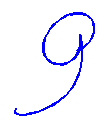
\includegraphics[height=0.12\textwidth]{figures/g4.png}}}
\subfigure{\raisebox{-0.5\height}{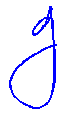
\includegraphics[height=0.12\textwidth]{figures/g5.png}}}
\caption[Sample letters generated from the PCA shape model on 120 `e' and `g'
paths.]{\label{fig:sampleLetters}Sample letters generated from the PCA shape
model on 120 `e' (top) and `g' paths (bottom), generated randomly from
parameters with $3\times$ the standard deviation observed in the dataset.}

\end{figure}

It is therefore feasible that `poor' letters can be produced using the shape
model generated from a dataset of adults' writing with PCA. In
\cite{Chandra2013}, it was found that children aged 4-6 participating in a
handwriting peer tutoring pilot study most often made mistakes classified as
inappropriate \emph{internal proportions} or \emph{global deformations}, and it
would be reasonable to consider the shapes in Figure \ref{fig:sampleLetters} in
the same general categories. Consequently, while using a database of children's
letters when available may yield potential for parameterising other mistakes
made by children, such as merging strokes or decomposing a shape into multiple
subparts inappropriately, sufficient capabilities for the shape model to
generate shapes given parameter variations which are appropriate for simulating
a na\"ive learning in the context of handwriting have been demonstrated.


\subsection{Responding to Feedback}

In the same way that the shape model of a particular letter can be used to take
parameters and generate a letter, in the case of the statistical shape model
presented in Section \ref{sec:writingGeneration}, it may also be used to take a
letter and determine its parameters given the model. The potential for the
parameters of a user-drawn shape to be obtained from the shape model have been
capitalised on to incorporate the capabilities for the learning algorithm to
adapt to the user's feedback via demonstration.

The statistical shape model may be used to determine the parameters of a
demonstration shape by projecting the features of the observed shape into the
lower-dimensional space determined by the model. Mathematically, given a
demonstration ${\bf x}$, the associated parameters may be determined as in
(\ref{eq:param}).

\begin{equation}\label{eq:param}
{\bf p}_{demo} ={\bf \Phi}^T ({\bf {x}-\bar{x}})
\end{equation}

The parameters which are determined for a shape will not reconstruct the shape
exactly, but rather will reconstruct the closest point in the N dimensional
space which the eigenvectors span. With increasing value of N, the reconstructed
shape will be closer to the original shape, until N is equal to the number of
dimensions of the original shape, at which point there is no error incurred by
`projecting' onto the N dimensional space as the space is the same (but perhaps
with a different basis).

For the statistical shape model employed by the system, the method for
responding to user demonstrations is to move the learning algorithm's parameters
towards those of the demonstration to some extent. In the results presented in
this work, \[{\bf p}^{(k+1)} = {\bf p}^{(k)} + ({\bf p}_{demo}-{\bf
p}^{(k)})\times\alpha\] has been used, where ${\bf p}$ is the parameter vector
and $k$ is the time step, and $\alpha$ is the learning rate, between 0 and 1.
While it is possible that the resulting ${\bf p}^{(k+1)}$ yields an unacceptable
shape from combining ${\bf p}^{(k)}$ and ${\bf p}_{demo}$ which individually
yield acceptable shapes, what is significant about the proposed method for
adapting to user demonstration is that even it does not get stuck at such poor
shapes: with further demonstrations of the same letter, the system would
eventually approach it. It remains to be seen what the impact of such a poor
in-between shape being drawn by the teachable agent would have on the
interaction with the user, however, and how - if necessary - to avoid such an
event mathematically.

Further research may discover how to best model/limit the learning speed of the
robot so that it is noticeably learning while not improving so fast as to limit
the long-term interaction potential for the system, which may turn out to be
child-dependent.

Figure \ref{fig:demonstrationShapes2} illustrates the response of the system to
demonstrations from a child for the letter `u' using a learning rate of
$\alpha=1/2$. 

\begin{figure}[thpb]
    \centering
    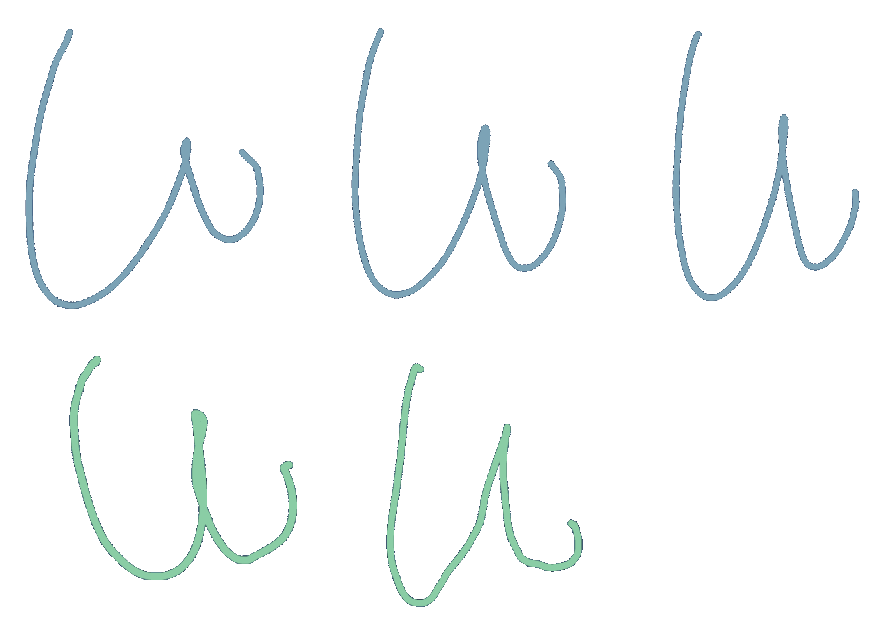
\includegraphics[width=0.3\textwidth]{figures/u_kids.png}
    \caption{\label{fig:demonstrationShapes2}Example of the learning algorithm
    responding to user demonstration of shapes for the letter `u.'}
\end{figure}





%%%%%%%%%%%%%%%%%%%%%%%%%%%%%%%%%%%%%%%%%%%%%%%%%%%%%%%%%%%%%%%%%%%%%%%%%%%%%%%%
\section{An Embodied Handwriting Learning Agent with the Nao Humanoid Robot} \label{sec:robotWriting}

In order to develop a teachable agent that is appropriate for engaging a child
through the learning by teaching paradigm - that is, that it is an embodied
agent, capable of eliciting motor mimicry, and capable of causing its teacher to
reflect on the process that has been used to respond to handwriting feedback -
capabilities for the robot to engage in handwriting have been established.

The Nao humanoid robot, which has been developed by Aldebaran-Robotics and
designed purposely to look approachable \cite{Gouaillier2008}, has been used for
this work. It is a commercially affordable biped robot, 58cm tall, with 25
degrees of freedom, two cameras, speech capabilities and the ability to
autonomously execute a range of tasks.

Because of the challenges in getting the Nao to write trajectories smoothly
because of its inherent ability to only reach discrete points in space, it has
been implemented instead that the robot uses simulated handwriting, as an
opportunity to have finer control over the robot's writing. The necessary
components to accomplish such are to:

\begin{enumerate}
    \item develop capabilities for the robot to trace handwriting, 

    \item synchronise the robot's movements with the display of the writing on a
        tablet so that it seems that the robot is causing the handwriting to
        display because of its actions, and

    \item integrate the writing behaviour with the handwriting learning
        algorithm presented in Section \ref{sec:learningAlgorithm} to create a
        learning by teaching interaction with the agent. 
\end{enumerate}

These steps are presented in the sections that follow.

\subsection{Robot Trajectory Following}

As previously mentioned, the robot used in this system does not have
capabilities to reach all points in space due to its physical limitations
(finite degrees of freedom). Using simulated handwriting will not do anything to
fix this physical limitation, but it provides a context where the path traced by
the robot can be displayed smoother than it would have otherwise appeared if
written with a writing instrument. For believability, however, it is still
necessary that the robot's trajectory is close enough to that which is
displayed. As such, the requirements on the robot's fine motor skills are
lessened but not removed. 

Aldebaran's NaoQi API has been used for the inverse kinematics of the trajectory
following. It provides the advantage of allowing the whole body to be used in
the inverse kinematics rather than simply the arm, which yields to an increased
working space of the robot. However, as motion planning is performed with
respect to the centre of the hand of the robot as opposed to the tip of a
writing instrument, restrictions on the orientation of the hand must be put in
place such that the writing instrument remains with the appropriate orientation
to the writing surface.

When pretending to write with a writing instrument, the requirement that the
instrument tip match the trajectory is still significant, and therefore any
change in orientation of the hand is exaggerated at the writing tip. 

Rather than have the robot write with a writing instrument on a horizontal
surface, by instead having it point at a vertical writing surface to cause the
trajectory to appear (as in Figure \ref{fig:naoWriting}), several advantages are
presented:

\begin{itemize}

    \item The working space of the robot increases, both in the technical sense
        and the interaction sense: someone can, in theory, show the tablet to
        the robot from across the room and have it still respond, without
        needing the tablet to be within arm's reach.

    \item Concerns about whether or not the child would start mimicking the
        robot's incorrect (inhuman) writing style are mitigated. However, there
        is a possibility that this would also reduce the potential for students
        to benefit from motor imitation, although it is hypothesised that motor
        imitation is caused more from the overall concept of the trajectory
        being shown than from the pen grip being used. 

    \item Perhaps most significantly, the accuracy of the matching of the
        robot's motion with the trajectory displayed on the tablet is not as
        critical, because the finger is not expected to touch the tablet exactly
        at the trajectory point, in contrast to the pen tip. This means that
        orientation degrees of freedom can be freed without significant adverse
        effects.

\end{itemize}

\begin{figure}[thpb]
     \begin{center}
        %\subfigure{
        %    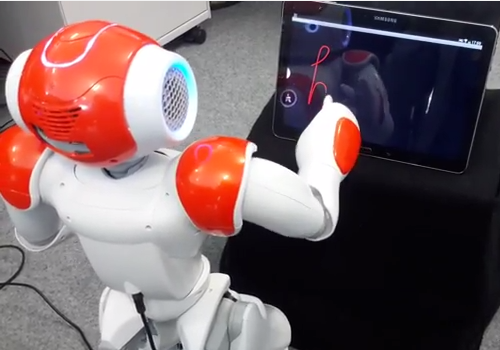
\includegraphics[width=0.4\textwidth]{figures/naoWriting1.png}
        %}%
        \subfigure{
            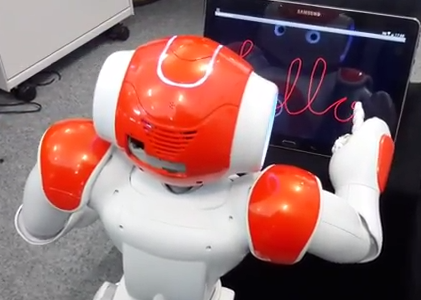
\includegraphics[width=0.3\textwidth]{figures/naoWriting2.png}
        }%
%
    \end{center}
    \caption{A demonstration of the robot simulating the drawing of a word
        with its finger, synchronised with the tablet, communicating over ROS.
     }%

   \label{fig:naoWriting}
\end{figure}

Therefore the system presented utilises the context where the robot is
simulating handwriting by pointing at the tablet\footnote{Teachers interviewed
for their feedback on the system advised that children are asked to draw letters
in the air in a similar manner as part of their handwriting education.}.

\subsection{Synchronisation with the Tablet Trajectory Display}

After getting the robot to trace writing trajectories, the next step towards
simulated handwriting is getting the trajectories of the robot's `writing' to
display on an Android tablet instead of being displayed in the RViz
visualisation tool running on the computer. 

ROS has been used to connect the devices used in the system, including the
Android tablet\footnote{For more information about ROS on Android devices see
\url{http://wiki.ros.org/android}}. As a result, aspects of the networking
between the tablet and the robot, such as the overheads associated with
connections, ports, message formats, publishers/subscribers, etc. have already
been implemented. 

An Android application has been developed to receive the trajectory message over
a ROS topic and add each point of the trajectory one by one as a frame of an
animation. Synchronisation between the tablet and the robot has been achieved by

\begin{itemize}

    \item sending a requested start time accompanying the trajectory, which is
        sufficiently in the future, to account for varying transmission delays
        to the nodes on different devices,

    \item synchronising all clocks with NTP servers such that the ROS time used
        for responding to the requested start time is the same at all nodes,

    \item reducing the number of points along the trajectory passed to the
        robot's motion planner, as the more points, the more the robot gets out
        of synch with the requested timings, and

    \item not running computationally expensive tasks on the robot (such as
        camera publishing) while it is writing, as this interferes with the
        requested timings between points. 

\end{itemize}

%\subsection{Integration and Synchronisation}

To instruct the robot where to write, the robot has been configured to detect a
particular fiducial marker, a \emph{chilitag}\footnote{See
\url{https://github.com/chili-epfl/ros_markers} for more information on the
fiducial marker detection node used.}, with the camera located in its head and
use that as the origin of the writing surface (Figure
\ref{fig:tabletDetection}). As publishing the robot's camera has been identified
as a computationally expensive task that can disrupt the robot's timing of
synchronised writing, it is only done when necessary and the tablet is assumed
to be stationary during the writing process.

\begin{figure}[htpb]
    \centering
    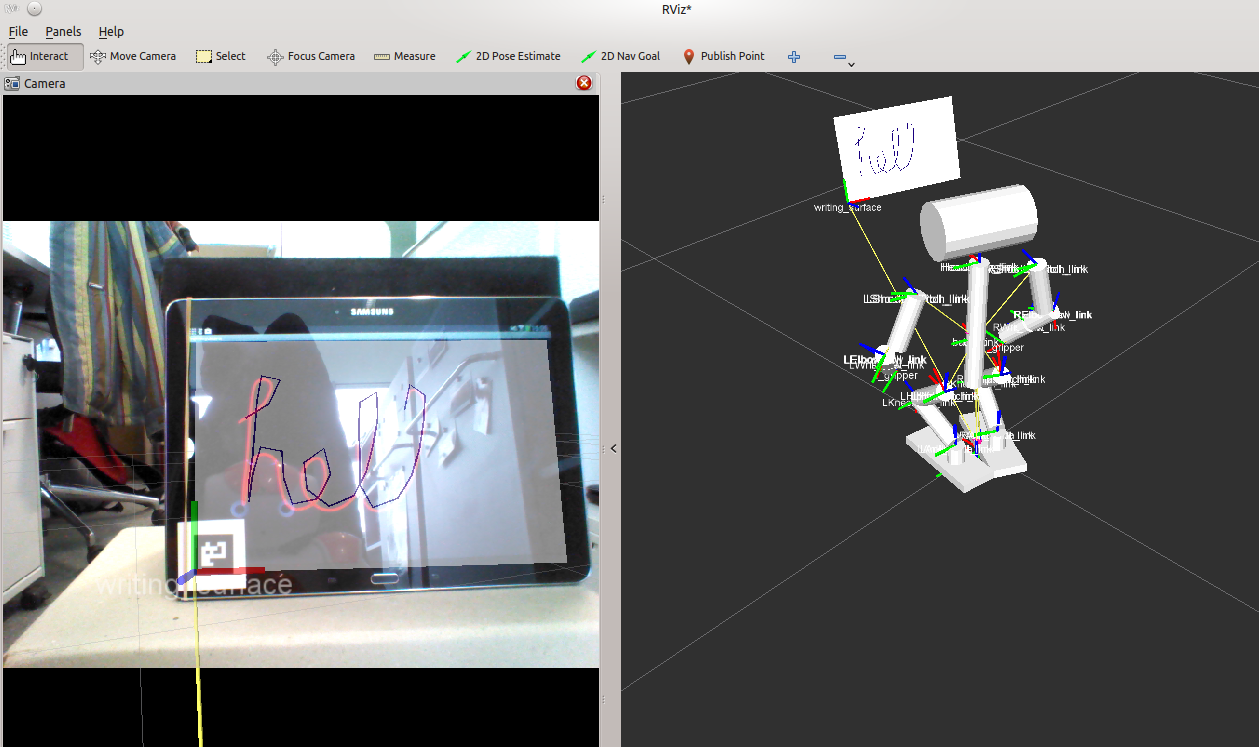
\includegraphics[width=0.45\textwidth]{figures/chilitagDetection_cameraOverlay.png}
    \caption[Detection of the tablet using a chilitag to represent the origin of
    the writing surface frame.]{\label{fig:tabletDetection}Detection of the
    tablet using a chilitag to represent the origin of the writing surface frame
(left: robot's camera image, with markers overlaid).}

\end{figure}


A demonstration of the robot executing a trajectory in synch with the tablet is
shown in Figure \ref{fig:naoWriting}\footnote{See
\url{https://www.youtube.com/watch?v=2qWFSJRxCU0} for a video of the
demonstration. }. As a result, the two relevant orientations of the hand were
fixed to keep the finger perpendicular to the writing surface, with the
remaining orientation free such that the wrist could rotate in order to easier
reach the points along the path. The use of whole body motion may be seen in
this demonstration, as the robot's centre of gravity is shifted to prevent the
wrist from rotating towards the centre of the robot, in which case the fingertip
would not match the writing trajectory. Without whole body motion control, it
would not have been possible to execute such a trajectory using only the degrees
of freedom in the arm.


\subsection{Integration into a Robotic Handwriting Learning Agent}

The fusion of the handwriting learning algorithm presented in Section
\ref{sec:learningAlgorithm} with the embodied handwriting agent developed
involves the integration of three components: the controller of the learning
algorithm, running on a computer, which manages the learning algorithm,
responding appropriate to feedback received, and publishes the shapes to be
drawn with their time and relevant position with respect to the writing surface;
the robot which draws the requested letters; and the application running on an
Android tablet which draws the requested letters in synch with the robot and
displays the result to the user, and acts as the medium for the user's feedback,
through touch gestures and user-drawn demonstrations.

Feedback from the user is passed to the controller with the location on the
tablet that it occurred at, and the task of interpreting the shape which the
feedback was intended for is left to the controller as it is aware of the
location of published shapes. The appropriate response in terms of the learning
algorithm is then taken for the respective shape. 

%%%%%%%%%%%%%%%%%%%%%%%%%%%%%%%%%%%%%%%%%%%%%%%%%%%%%%%%%%%%%%%%%%%%%%%%%%%%%%%%

%%%%%%%%%%%%%%%%%%%%%%%%%%%%%%%%%%%%%%%%%%%%%%%%%%%%%%%%%%%%%%%%%%%%%%%%%%%%%%%%

\section{A Tool for Social and Pedagogical Investigations} \label{sec:experiment}

In addition to constituting a technically novel system, the teachable robotic
agent presented represents a tool which may be used for investigating social and
pedagogical research questions. One such question that is being worked towards
is what impact to the outcomes of a handwriting intervention the addition of
such a teachable robotic agent would have. 

%\subsection{Interaction Context}

The interaction context which has been developed as a framework for addressing
such questions is one where participants are asked to improve the robot's
handwriting by correcting its letters. Figure \ref{fig:pilotInteraction}
illustrates an example interaction sequence between the participant and the
robot, which consists of the following stages.

\begin{enumerate}

    \item The participant shows the robot one of five different 3-letter words
        to write, which, combined, consist of 7 different letters (`c', `e',
        `n', `o', `s', `u', `w'). Fiducial markers placed on the word cards to
        allow for detection with a camera. 

    \item The robot responds to the word request verbally and writes the letters
        by pointing at the tablet - placed in front of it with a vertical
        orientation - and imitating tracing the letters as they appear
        simultaneously by being displayed by the tablet. 

    \item The robot asks for feedback from the participant and they demonstrate
        how to write the letter which they feel needs to be corrected. The
        demonstration is performed by drawing on the tablet with a stylus,
        either with the tablet still in a vertical orientation or by unfolding
        the stand and laying the tablet flat on the desk. The position of the
        participant's demonstration on the tablet encodes the shape letter that
        it is a demonstration for. The participant can clear their shapes if
        they are unhappy with them or they are in the wrong position. When the
        button to signal that it is the robot's turn is pressed, the
        demonstration is sent to the controller.

    \item The interaction iterates, with participants taking turns to interact
        with the robot.

\end{enumerate}

%To allow the system to take input from the user on which words to draw,
%fiducial markers were placed on cards which were detectable by a
%previously-developed ROS node processing a camera stream. A node which
%processed the fiducial markers detected was then created to convert the card
%detected into an appropriate message for the controller. 
	
\begin{figure}[thpb!]
     \begin{center}
%
        \subfigure[The user shows a card to the robot with a word to write.]{%
            \label{fig:first}
            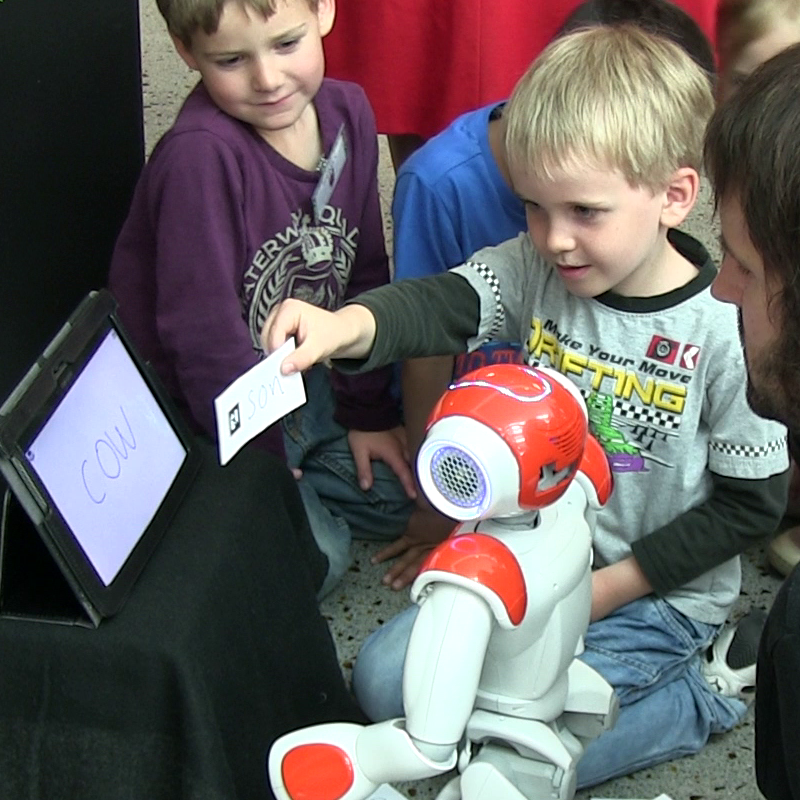
\includegraphics[width=0.2\textwidth]{figures/1card.png}
        }~
        \subfigure[The robot writes the word seen on the card and asks for feedback.]{%
           \label{fig:second}
           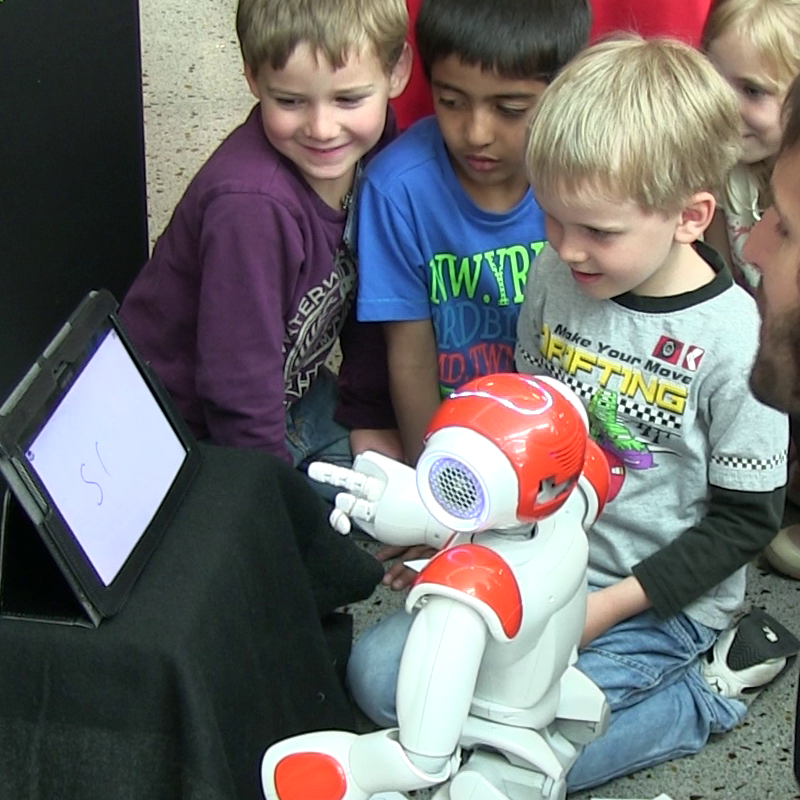
\includegraphics[width=0.2\textwidth]{figures/2word.png}
        }\\ %  ------- End of the first row ----------------------%
        \subfigure[The user provides feedback on the letters written via demonstration.]{%
            \label{fig:third}
            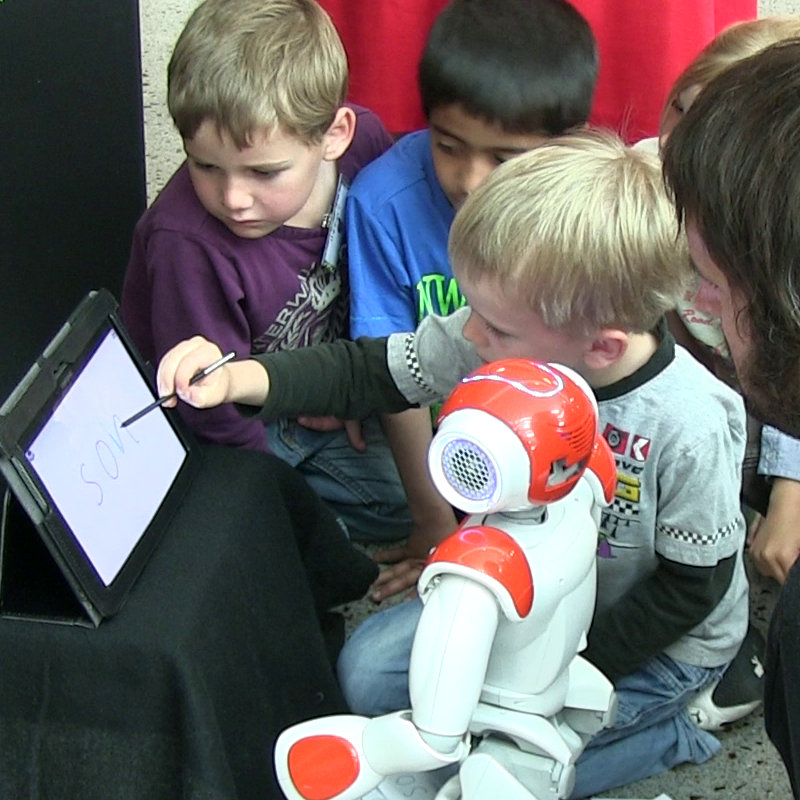
\includegraphics[width=0.2\textwidth]{figures/4correct.png}
        }~
        \subfigure[The robot responds to the feedback and asks for more.]{%
            \label{fig:fourth}
            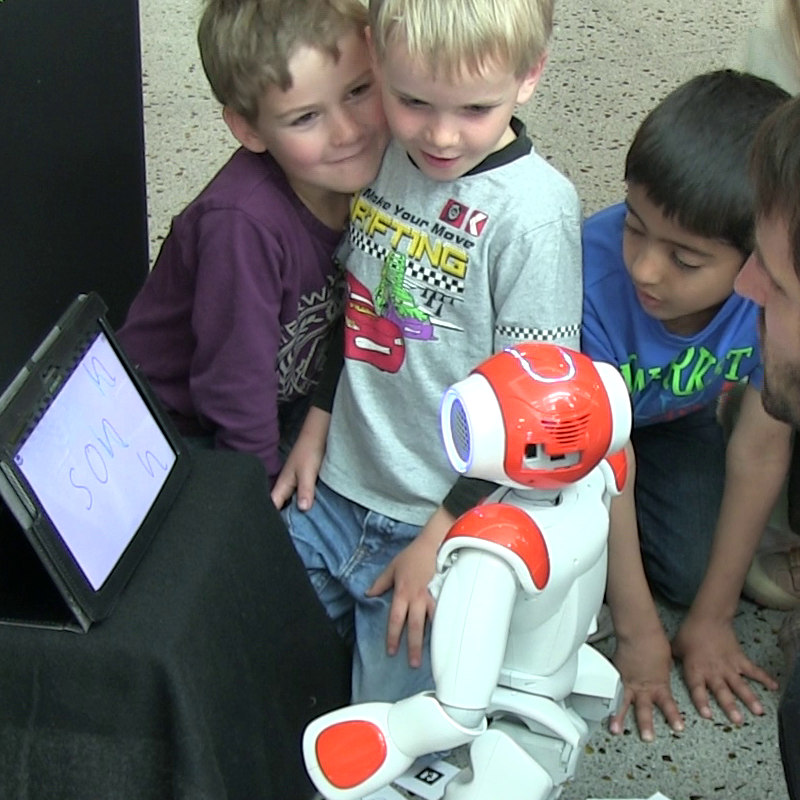
\includegraphics[width=0.2\textwidth]{figures/5iterateAsk.png}
        }%
%
    \end{center}
    \caption{%
        A user interacting with the robot in the learning by teaching interaction using demonstrations.
     }%
   \label{fig:pilotInteraction}
\end{figure}

%\subsection{Outcomes}

A pilot study has been conducted to evaluate the interaction in preparation for
an experiment to be conducted on the 10th-11th of June, 2014. The pilot study
consisted of four groups of approximately 8 children, aged 6-7 years. Outcomes
from the pilot study include information on how children interact with the
system, sample letters written by children, opinions from the teachers involved,
and insight into what experimental conditions might be appropriate for the
experiment. 

The system was validated, in that the learning algorithm and robotic writing
were believed by the children, and that the system withstood the interaction for
a total of 65 minutes, with the robot writing 96 letters, 49 of which in
response to demonstrations from the children, during that time. 

Another key point which came from the pilot study is that children were observed
giving advice to the child designated as the letter demonstrator, potentially
giving rise to the higher level paradigm of learning by \emph{teaching to
teach}. 

%\begin{itemize}
%
%\item Children would not intuitively write over the robot's letters, but rather
%above them. When instructed to write over the robot's letter, some participants
%would trace the letter as it had previously appeared as their demonstration. As
%such, the requested demonstration positioning will be modified for the
%experiment.
%
%\item While children spoke to the robot each time it requested feedback -
%suggesting that the anthropomorphised the robot - they also laughed when it
%wrote letters which were incorrect, which may suggest that they had not
%developed an empathetic connection with the robot by that point. 
%
%\item Children were observed giving advice to the child designated as the
%letter demonstrator, potentially giving rise to the higher level paradigm of
%learning by teaching to teach. 
%
%\end{itemize}

As a consequence of this observation, the upcoming experiment will address the
effect of the number of children interacting with the robot in order to
investigate the potential of the system to not only be used to set the context
of children tutoring the robot, but also children interacting as peer tutors
with each other.


%\section{ADDITIONAL REQUIREMENTS}


%%%%%%%%%%%%%%%%%%%%%%%%%%%%%%%%%%%%%%%%%%%%%%%%%%%%%%%%%%%%%%%%%%%%%%%%%%%%%%%%
\section{Conclusions and Future Work}

%\subsection{Conclusions}

The technical challenges involved in developing a teachable robotic agent in the context of handwriting which have been addressed in this work include:

\begin{itemize}

    \item developing capabilities for a robot with limited fine motor
        capabilities, such as the Nao, to engage in the act of handwriting in a
        way that is believable for interacting with children, which has been
        accomplished by leveraging simulated handwriting with a synchronised
        tablet;

    \item developing a system for generating poorly written letters appropriate
        for simulating a na\"ive learner in the context of handwriting, achieved
        by using statistical shape models through PCA of observations of the
        trajectory of the same letter;

    \item developing an algorithm capable of incorporating user feedback and
        demonstrations in order to adapt the generated handwriting quality so as
        to simulate a teachable agent, which has been implemented by maintaining
        a learning algorithm in the parameter space of the shape models and
        converging towards the parameters of user demonstrations; and

    \item integrating the system into a working interaction suitable for
        engaging children in the learning by teaching paradigm, accomplished by
        fusing the robotic drawing capabilities and the learning algorithm for
        handwritten letters established.

\end{itemize}

%By leveraging the technology of a wirelessly synchronised tablet displaying a
%writing trajectory, the requirements for a robot with limited fine motor
%capabilities to accurately manipulate a writing implement have been reduced to
%instead requiring that the robot roughly trace the trajectory as it is
%simultaneously displayed on the tablet. Thus, capabilities for the Nao to
%engage in simulated handwriting have been demonstrated. By further lifting the
%constraint that the robot must draw with a writing instrument and allowing it
%instead to draw with its finger, in addition to increasing the range of
%trajectories which the robot is able to reach, the necessary accuracy in the
%robot's trajectory following is reduced as it is not necessary for the finger
%to physically touch the writing surface at the trajectory position for the
%simulation to be believable. As the motion control is currently limited to the
%position of the robot's hand rather than the writing tip, the reduced need for
%accurate motion in order to have a believable simulation was leveraged upon in
%the presented system to produce results with the robot drawing with its finger
%of sufficient accuracy. 

%Statistical shape modeling using principal component analysis on a dataset of
%writing trajectories for a letter has been employed to generate shape models of
%different letters/allographs. These models, generated through unsupervised
%methods, have been shown to capture the internal proportions of letters in a
%similar way to how human intuition would identify the possible shape variances
%(width/height/proportional size of loops, skewness, etc.). As a result, the
%models have been used to generate synthetic letters which yield shapes
%appropriate for use in an artificial intelligence algorithm which uses user
%feedback on the best letter from a set of candidates drawn to converge to the
%parameter values of the selected shapes after some iterations.

%The letter model has been used to determine the parameter values of shapes
%demonstrated by the user. Provided that the user demonstrates the shape in the
%same style as those used to generate the shape model (i.e., with the strokes in
%the appropriate order and direction), the parameters of the demonstration may
%then be used as input to the learning algorithm to converge towards the user's
%writing demonstrations. 

%The fusion of the robotic drawing capabilities and the learning algorithm for
%handwritten letters has resulted in a teachable robotic agent which can engage
%users in the learning by teaching paradigm in the context of handwriting. As
%such, the system developed has been shown to accomplish the technical goals
%which were set out to be achieved, and the implications of such a system
%evaluation of the system is underway, with an in situ interaction with primary
%school students being conducted in the coming weeks. 

The work presented opens up the research area of the role for robots in the
education of handwriting and other embodied activities, and makes significant,
novel steps towards addressing the over-arching research question of how
interacting with such a robotic learning partner may be beneficial for
sustaining a child's interaction in handwriting interventions and the impact on
the participating child's motivation, self-esteem, and educational future.


%\subsection{Future Works}
%\section{Future work}

%A number of research questions remain open for investigation in the wider scope
%of the CoWriter project, in addition to those which have been raised as a
%result of the work carried out to develop the presented system.

%In the scope of open technical questions, it remains to be seen how shape
%models for letters might be generated which capture the full range of mistakes
%typical of children learning handwriting: extending the current system capable
%of incorporating internal proportion and global deformation errors to one which
%can also generate missing subparts of the letter, or break the letter down into
%primitive strokes at will, for example. Could incorporating a database of
%letters drawn by children into the shape modeling process facilitate this? 

%In terms of the interaction experience, it may be interesting to investigate
%which other technology could be incorporated into the system for a more fluid
%interaction, such as integrating the user's gaze information to infer when the
%user is finished with a demonstration, or using a classification algorithm to
%determine which letter has been demonstrated irrespective of its positioning.

%On the educational side, open questions include how the handwriting error
%generation of the system may be abstracted to a higher level of control so that
%a teacher may configure it to work with a child on a particular type of
%mistakes, based on the child's performance. Where would the balance lie between
%developing autonomous capabilities for the system to determine the child's
%difficulties, and empowering the teaching staff to decide for themselves
%instead? And, as a result, the ultimate question for this area of research is
%to address what impact to the outcomes of a handwriting intervention the
%addition of such a teachable robotic agent would have: does it impact the
%motivation of the participants, their self-esteem, and/or the learning gains
%that they experience?

%%%%%%%%%%%%%%%%%%%%%%%%%%%%%%%%%%%%%%%%%%%%%%%%%%%%%%%%%%%%%%%%%%%%%%%%%%%%%%%%
%%\section{ACKNOWLEDGMENTS}

%The authors gratefully acknowledge the contribution of National Research Organization and reviewers' comments.


%%%%%%%%%%%%%%%%%%%%%%%%%%%%%%%%%%%%%%%%%%%%%%%%%%%%%%%%%%%%%%%%%%%%%%%%%%%%%%%%

%\begin{thebibliography}
\bibliographystyle{abbrv}
\bibliography{library}

%\end{thebibliography}

\end{document}
